\scanpage{21}
% Diplomatic reading A. Literal source groups use fixed image-coordinate origins;
% .055mm per source pixel, negative y direction. Manual geometric approximations,
% source-only validation; no compilation, rendering or metric fit is claimed.
Soit $\alpha_0\in K_1$, je dis que \unsure{l'on a|on a}
\[
\unsure{% head-arm/independent upper-run role remains open; Sigma reading retained
% A021G01 BEGIN; source bbox=[566, 155, 693, 257]; source origin=(566,155); baseline y=226; owns: complete Sigma, its separate head, index and any raised sign/hat; no adjoining relation or word
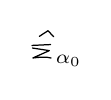
\begin{tikzpicture}[x=.055mm,y=-.055mm,baseline=(A021G01base),line cap=round,line join=round]
\path[use as bounding box] (566,155) rectangle (693,257);
\coordinate (A021G01base) at (566,226);
% invisible complete reading/state annotation: \widehat\Sigma_{\alpha_0}
\node[overlay,anchor=base west,inner sep=0pt,outer sep=0pt] at (566,226) {\phantom{$\widehat\Sigma_{\alpha_0}$}};
\draw[line width=.45pt] (576,196)--(619,194);
\draw[line width=.45pt] (577,202)--(616,208)--(578,225)..controls(592,223)and(610,222)..(620,225);
\draw[line width=.45pt] (593,175)--(613,162)--(626,176);
\node[anchor=base west,inner sep=0pt,outer sep=0pt] at (631,238) {$\scriptstyle\alpha_0$};
\end{tikzpicture}
% A021G01 END
}
\cap% A021G02 BEGIN; source bbox=[735, 155, 837, 241]; source origin=(735,155); baseline y=225; owns: complete Sigma, its separate head, index and any raised sign/hat; no adjoining relation or word
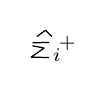
\begin{tikzpicture}[x=.055mm,y=-.055mm,baseline=(A021G02base),line cap=round,line join=round]
\path[use as bounding box] (735,155) rectangle (837,241);
\coordinate (A021G02base) at (735,225);
\draw[line width=.45pt] (747,190)--(784,189);
\draw[line width=.45pt] (747,197)--(773,202)--(743,223)--(783,224);
\draw[line width=.45pt] (757,175)--(776,161)--(790,175);
\node[anchor=base west,inner sep=0pt,outer sep=0pt] at (793,234) {$\scriptstyle i$};
\node[anchor=base west,inner sep=0pt,outer sep=0pt] at (807,202) {$\scriptstyle+$};
\end{tikzpicture}
% A021G02 END
=\varnothing\qquad\text{\unsure{i.e|i.e.}}\qquad% A021G03 BEGIN; source bbox=[1236, 178, 1328, 250]; source origin=(1236,178); baseline y=225; owns: complete Sigma, its separate head, index and any raised sign/hat; no adjoining relation or word
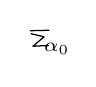
\begin{tikzpicture}[x=.055mm,y=-.055mm,baseline=(A021G03base),line cap=round,line join=round]
\path[use as bounding box] (1236,178) rectangle (1328,250);
\coordinate (A021G03base) at (1236,225);
\draw[line width=.45pt] (1242,185)--(1285,184);
\draw[line width=.45pt] (1244,192)--(1274,199)--(1248,221)--(1284,219);
\node[anchor=base west,inner sep=0pt,outer sep=0pt] at (1274,234) {$\scriptstyle\alpha_0$};
\end{tikzpicture}
% A021G03 END
\cap% A021G04 BEGIN; source bbox=[1337, 178, 1400, 244]; source origin=(1337,178); baseline y=226; owns: complete Sigma, its separate head, index and any raised sign/hat; no adjoining relation or word
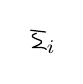
\begin{tikzpicture}[x=.055mm,y=-.055mm,baseline=(A021G04base),line cap=round,line join=round]
\path[use as bounding box] (1337,178) rectangle (1400,244);
\coordinate (A021G04base) at (1337,226);
\draw[line width=.45pt] (1344,184)--(1378,188);
\draw[line width=.45pt] (1357,191)..controls(1340,197)and(1346,200)..(1368,208)..controls(1375,215)and(1355,220)..(1348,224)..controls(1365,223)and(1376,223)..(1380,228);
\node[anchor=base west,inner sep=0pt,outer sep=0pt] at (1381,237) {$\scriptstyle i$};
\end{tikzpicture}
% A021G04 END
=\varnothing
\]
(ce qui ach\unsure{è|é|e}vera la d\unsure{è|é}monstration, car on aura
\figure{\unsure{% two pale interrupted traces; role, hand and surface origin unresolved
% A021M01 BEGIN; source bbox=[834, 415, 892, 448]; source origin=(834,415); baseline y=440; owns: two faint traces only; aura and both displays outside
\begin{tikzpicture}[x=.055mm,y=-.055mm,baseline=(A021M01base),line cap=round,line join=round]
\path[use as bounding box] (834,415) rectangle (892,448);
\coordinate (A021M01base) at (834,440);
\draw[gray!70,line width=.2pt] (840,421)--(848,423) (852,423)--(861,425) (865,426)--(878,428);
\draw[gray!70,line width=.2pt] (841,436)--(849,438) (854,438)--(864,440) (868,441)--(887,443);
\end{tikzpicture}
% A021M01 END
}
}
\[
U=X\setminus\bigcup_{\alpha\in K}
% A021G05 BEGIN; source bbox=[896, 469, 1018, 563]; source origin=(896,469); baseline y=535; owns: complete Sigma, its separate head, index and any raised sign/hat; no adjoining relation or word
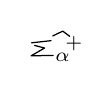
\begin{tikzpicture}[x=.055mm,y=-.055mm,baseline=(A021G05base),line cap=round,line join=round]
\path[use as bounding box] (896,469) rectangle (1018,563);
\coordinate (A021G05base) at (896,535);
\draw[line width=.45pt] (905,504)--(950,499);
\draw[line width=.45pt] (912,510)--(935,516)--(904,534)--(955,533);
\draw[line width=.45pt] (954,488)--(977,477)--(993,489);
\node[anchor=base west,inner sep=0pt,outer sep=0pt] at (960,546) {$\scriptstyle\alpha$};
\node[anchor=base west,inner sep=0pt,outer sep=0pt] at (983,517) {$\scriptstyle+$};
\end{tikzpicture}
% A021G05 END
\qquad% A021G18 BEGIN; source bbox=[1103, 401, 1480, 635]; source origin=(1103,401); baseline y=543; owns: K=K1 union {i}, incomplete-top-arm main brace, and nested complete cancelled group; no U formula
\begin{tikzpicture}[x=.055mm,y=-.055mm,baseline=(A021G18base),line cap=round,line join=round]
\path[use as bounding box] (1103,401) rectangle (1480,635);
\coordinate (A021G18base) at (1103,543);
\draw[line width=.4pt] (1135,418)..controls(1133,458)and(1131,492)..(1128,526)..controls(1126,547)and(1120,555)..(1115,555)..controls(1110,552)and(1107,548)..(1109,551)..controls(1125,560)and(1122,574)..(1119,601)..controls(1118,615)and(1118,627)..(1121,632);
\node[anchor=base west,inner sep=0pt,outer sep=0pt] at (1160,447) {$K=K_1\cup\{i\}$};
\node[anchor=base west,inner sep=0pt,outer sep=0pt] at (1137,532) {$\unsure{% cancelled Sigma-alpha candidate; index remains uncertain
% A021G19 BEGIN; source bbox=[1137, 484, 1246, 547]; source origin=(1137,484); baseline y=532; owns: cancelled Sigma and alpha, all crossing strokes; K condition and main brace outside
\begin{tikzpicture}[x=.055mm,y=-.055mm,baseline=(A021G19base),line cap=round,line join=round]
\path[use as bounding box] (1137,484) rectangle (1246,547);
\coordinate (A021G19base) at (1137,532);
% invisible complete reading/state annotation: \deleted{\unsure{\Sigma_\alpha}}
\node[overlay,anchor=base west,inner sep=0pt,outer sep=0pt] at (1137,532) {\phantom{$\deleted{\unsure{\Sigma_\alpha}}$}};
\draw[line width=.35pt] (1150,499)--(1202,494);
\draw[line width=.35pt] (1152,505)--(1186,518)--(1143,529)--(1203,529);
\draw[line width=.55pt] (1141,526)--(1172,490)--(1202,492)--(1164,525)--(1215,510)--(1177,535)--(1230,515)--(1201,538);
\node[anchor=base west,inner sep=0pt,outer sep=0pt] at (1220,541) {$\scriptstyle\alpha$};
\end{tikzpicture}
% A021G19 END
}
$};
\end{tikzpicture}
% A021G18 END
\]
comme dans le lemme.

Or \unsure{comme|\deleted{co}mme} on a
\margin{\unsure{% pale oblique trace; role, hand and surface origin unresolved
% A021M02 BEGIN; source bbox=[102, 880, 122, 901]; source origin=(102,880); baseline y=895; owns: isolated left-margin tick only
\begin{tikzpicture}[x=.055mm,y=-.055mm,baseline=(A021M02base),line cap=round,line join=round]
\path[use as bounding box] (102,880) rectangle (122,901);
\coordinate (A021M02base) at (102,895);
\draw[gray,line width=.2pt] (109,892)--(116,886);
\end{tikzpicture}
% A021M02 END
}
}
\[
E_i\subset U_{J,i}=X\setminus
% A021G06 BEGIN; source bbox=[1000, 849, 1148, 984]; source origin=(1000,849); baseline y=925; owns: complete cup, crossing high stroke and lower limit; preceding X/setminus outside
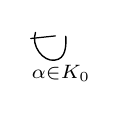
\begin{tikzpicture}[x=.055mm,y=-.055mm,baseline=(A021G06base),line cap=round,line join=round]
\path[use as bounding box] (1000,849) rectangle (1148,984);
\coordinate (A021G06base) at (1000,925);
% invisible complete reading/state annotation: \bigcup_{\alpha\in K_0}
\node[overlay,anchor=base west,inner sep=0pt,outer sep=0pt] at (1000,925) {\phantom{$\bigcup_{\alpha\in K_0}$}};
\draw[line width=.5pt] (1018,860)..controls(1007,891)and(1036,928)..(1062,924)..controls(1089,922)and(1089,889)..(1088,869);
\draw[line width=.45pt] (1007,874)--(1064,868);
\node[anchor=base west,inner sep=0pt,outer sep=0pt] at (1009,966) {$\scriptstyle\alpha\in K_0$};
\end{tikzpicture}
% A021G06 END
\unsure{% detached point and pale lower trace: role, hand and surface origin unresolved
% A021G07 BEGIN; source bbox=[1142, 831, 1241, 934]; source origin=(1142,831); baseline y=912; owns: complete Sigma, its separate head, index and any raised sign/hat; no adjoining relation or word
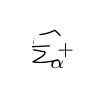
\begin{tikzpicture}[x=.055mm,y=-.055mm,baseline=(A021G07base),line cap=round,line join=round]
\path[use as bounding box] (1142,831) rectangle (1241,934);
\coordinate (A021G07base) at (1142,912);
\draw[line width=.45pt] (1153,875)--(1192,873);
\draw[line width=.45pt] (1155,882)--(1182,887)..controls(1186,894)and(1167,902)..(1154,910)..controls(1177,914)and(1205,907)..(1213,906);
\draw[line width=.45pt] (1170,847)..controls(1185,846)and(1199,840)..(1205,837)--(1217,849);
\fill (1157,856) circle[radius=.65];
\draw[gray,line width=.2pt] (1155,861)..controls(1153,864)and(1156,866)..(1155,869);
\node[anchor=base west,inner sep=0pt,outer sep=0pt] at (1194,926) {$\scriptstyle\alpha$};
\node[anchor=base west,inner sep=0pt,outer sep=0pt] at (1210,895) {$\scriptstyle+$};
\end{tikzpicture}
% A021G07 END
}
\]
cela implique que
\[
E_i\subset X\setminus
% A021G08 BEGIN; source bbox=[911, 1078, 1034, 1178]; source origin=(911,1078); baseline y=1152; owns: complete Sigma, its separate head, index and any raised sign/hat; no adjoining relation or word
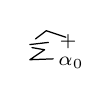
\begin{tikzpicture}[x=.055mm,y=-.055mm,baseline=(A021G08base),line cap=round,line join=round]
\path[use as bounding box] (911,1078) rectangle (1034,1178);
\coordinate (A021G08base) at (911,1152);
\draw[line width=.45pt] (916,1117)--(959,1112);
\draw[line width=.45pt] (921,1124)--(950,1129)--(916,1152)--(970,1150);
\draw[line width=.45pt] (929,1104)--(954,1085)--(999,1100);
\node[anchor=base west,inner sep=0pt,outer sep=0pt] at (982,1166) {$\scriptstyle\alpha_0$};
\node[anchor=base west,inner sep=0pt,outer sep=0pt] at (985,1122) {$\scriptstyle+$};
\end{tikzpicture}
% A021G08 END
=% A021G09 BEGIN; source bbox=[1132, 1098, 1280, 1181]; source origin=(1132,1098); baseline y=1150; owns: complete Sigma, its separate head, index and any raised sign/hat; no adjoining relation or word
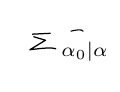
\begin{tikzpicture}[x=.055mm,y=-.055mm,baseline=(A021G09base),line cap=round,line join=round]
\path[use as bounding box] (1132,1098) rectangle (1280,1181);
\coordinate (A021G09base) at (1132,1150);
\draw[line width=.45pt] (1143,1113)--(1184,1111);
\draw[line width=.45pt] (1146,1119)--(1173,1127)--(1137,1149)..controls(1154,1147)and(1188,1142)..(1197,1147);
\draw[line width=.4pt] (1232,1106)..controls(1244,1103)and(1257,1101)..(1260,1106);
\node[anchor=base west,inner sep=0pt,outer sep=0pt] at (1210,1164) {$\scriptstyle\unsure{\alpha_0|\alpha}$};
\end{tikzpicture}
% A021G09 END
\]
% independent right-margin group; transverse labels run bottom-to-top.
\margin{\unsure{% complete candidates j:e., j.e., i:e., i.e.; two intermediate points present, attachment unresolved
% A021G20 BEGIN; source bbox=[1352, 1129, 1420, 1183]; source origin=(1352,1129); baseline y=1161; owns: complete small marginal lead-in including j dot, two intermediate points, e, final point; diagram outside
\begin{tikzpicture}[x=.055mm,y=-.055mm,baseline=(A021G20base),line cap=round,line join=round]
\path[use as bounding box] (1352,1129) rectangle (1420,1183);
\coordinate (A021G20base) at (1352,1161);
% invisible complete reading/state annotation: \text{j:e.}\mid\text{j.e.}\mid\text{i:e.}\mid\text{i.e.}
\node[overlay,anchor=base west,inner sep=0pt,outer sep=0pt] at (1352,1161) {\phantom{$\text{j:e.}\mid\text{j.e.}\mid\text{i:e.}\mid\text{i.e.}$}};
\draw[line width=.45pt] (1365,1149)..controls(1369,1161)and(1364,1171)..(1357,1176);
\draw[line width=.45pt] (1364,1133)--(1367,1139);
\fill (1378,1155) circle[radius=1.1];
\fill (1381,1161) circle[radius=1.1];
\draw[line width=.45pt] (1395,1144)..controls(1391,1148)and(1392,1155)..(1398,1160);
\fill (1410,1159) circle[radius=1.1];
\end{tikzpicture}
% A021G20 END
}
% A021DG BEGIN; complete marginal diagram; fixed source origin (1435,948).
\diagram{\begin{tikzcd}[ampersand replacement=\&,column sep=0pt,row sep=0pt,execute at end picture={
\begin{scope}[shift={(A021DGanchor.north west)},x=.055mm,y=-.055mm]
\begin{scope}[shift={(-1435,-948)}]
\node[anchor=base west,inner sep=0pt,outer sep=0pt] at (1505,994) {$% A021D01 BEGIN; source bbox=[1505, 957, 1582, 1015]; source origin=(1505,957); baseline y=994; owns: complete Sigma, its separate head, index and any raised sign/hat; no adjoining relation or word
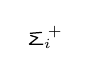
\begin{tikzpicture}[x=.055mm,y=-.055mm,baseline=(A021D01base),line cap=round,line join=round]
\path[use as bounding box] (1505,957) rectangle (1582,1015);
\coordinate (A021D01base) at (1505,994);
\draw[line width=.45pt] (1511,970)--(1537,968);
\draw[line width=.45pt] (1512,975)--(1528,980)--(1509,995)--(1540,995);
\node[anchor=base west,inner sep=0pt,outer sep=0pt] at (1542,1005) {$\scriptscriptstyle i$};
\node[anchor=base west,inner sep=0pt,outer sep=0pt] at (1551,975) {$\scriptscriptstyle+$};
\end{tikzpicture}
% A021D01 END
$};
\node[anchor=base west,inner sep=0pt,outer sep=0pt] at (1603,1000) {$% A021D02 BEGIN; source bbox=[1603, 961, 1665, 1017]; source origin=(1603,961); baseline y=1000; owns: complete Sigma, its separate head, index and any raised sign/hat; no adjoining relation or word
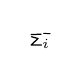
\begin{tikzpicture}[x=.055mm,y=-.055mm,baseline=(A021D02base),line cap=round,line join=round]
\path[use as bounding box] (1603,961) rectangle (1665,1017);
\coordinate (A021D02base) at (1603,1000);
\draw[line width=.45pt] (1611,977)--(1634,976);
\draw[line width=.45pt] (1612,982)--(1627,986)--(1611,1001)--(1635,1001);
\draw[line width=.35pt] (1640,974)--(1655,975);
\node[anchor=base west,inner sep=0pt,outer sep=0pt] at (1636,1010) {$\scriptscriptstyle i$};
\end{tikzpicture}
% A021D02 END
$};
\node[anchor=base west,inner sep=0pt,outer sep=0pt] at (1534,1118) {$\unsure{% Sigma_i-alpha / Sigma_i,alpha / Sigma_dot-alpha; point attachment and absent separate i-body remain open
% A021D03 BEGIN; source bbox=[1534, 1086, 1616, 1138]; source origin=(1534,1086); baseline y=1118; owns: third upright diagram Sigma, detached point and low alpha only
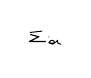
\begin{tikzpicture}[x=.055mm,y=-.055mm,baseline=(A021D03base),line cap=round,line join=round]
\path[use as bounding box] (1534,1086) rectangle (1616,1138);
\coordinate (A021D03base) at (1534,1118);
% invisible complete reading/state annotation: \Sigma_{i\alpha}\mid\Sigma_{i,\alpha}\mid\Sigma_{\dot\alpha}
\node[overlay,anchor=base west,inner sep=0pt,outer sep=0pt] at (1534,1118) {\phantom{$\Sigma_{i\alpha}\mid\Sigma_{i,\alpha}\mid\Sigma_{\dot\alpha}$}};
\draw[line width=.35pt] (1540,1097)--(1567,1094);
\draw[line width=.4pt] (1541,1102)--(1560,1107)--(1538,1118)--(1575,1118);
\fill (1582,1107) circle[radius=.9];
\draw[line width=.35pt] (1583,1120)..controls(1588,1113)and(1595,1114)..(1596,1120)..controls(1596,1125)and(1587,1125)..(1583,1121)..controls(1594,1124)and(1601,1119)..(1603,1115)..controls(1601,1122)and(1607,1125)..(1611,1124);
\end{tikzpicture}
% A021D03 END
}
$};
\node[anchor=base west,inner sep=0pt,outer sep=0pt] at (1518,1251) {$% A021D04 BEGIN; source bbox=[1518, 1206, 1640, 1279]; source origin=(1518,1206); baseline y=1251; owns: complete Sigma, its separate head, index and any raised sign/hat; no adjoining relation or word
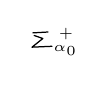
\begin{tikzpicture}[x=.055mm,y=-.055mm,baseline=(A021D04base),line cap=round,line join=round]
\path[use as bounding box] (1518,1206) rectangle (1640,1279);
\coordinate (A021D04base) at (1518,1251);
\draw[line width=.45pt] (1530,1218)--(1565,1216);
\draw[line width=.45pt] (1533,1224)--(1553,1231)--(1528,1251)--(1574,1249);
\node[anchor=base west,inner sep=0pt,outer sep=0pt] at (1578,1260) {$\scriptscriptstyle\alpha_0$};
\node[anchor=base west,inner sep=0pt,outer sep=0pt] at (1590,1228) {$\scriptscriptstyle+$};
\end{tikzpicture}
% A021D04 END
$};
\node[anchor=base west,inner sep=0pt,outer sep=0pt] at (1472,1165) {$\unsure{% upright ! on page / sideways ou / dash; selected point and curved stroke remain literal
% A021D05 BEGIN; source bbox=[1472, 1122, 1498, 1176]; source origin=(1472,1122); baseline y=1165; owns: middle transverse point and curved stroke only; both transverse Sigmas outside
\begin{tikzpicture}[x=.055mm,y=-.055mm,baseline=(A021D05base),line cap=round,line join=round]
\path[use as bounding box] (1472,1122) rectangle (1498,1176);
\coordinate (A021D05base) at (1472,1165);
% invisible complete reading/state annotation: \rotatebox{-90}{$!$}\mid\text{ou}\mid-
\node[overlay,anchor=base west,inner sep=0pt,outer sep=0pt] at (1472,1165) {\phantom{$\rotatebox{-90}{$!$}\mid\text{ou}\mid-$}};
\fill (1480,1156) circle[radius=.9];
\draw[line width=.4pt] (1487,1145)..controls(1487,1137)and(1487,1131)..(1491,1125);
\end{tikzpicture}
% A021D05 END
}
$};
\node[anchor=base west,inner sep=0pt,outer sep=0pt] at (1457,1260) {$\unsure{% short detached pale stroke; brace continuation, role, hand and surface origin open
% A021M04 BEGIN; source bbox=[1457, 1244, 1473, 1266]; source origin=(1457,1244); baseline y=1260; owns: short pale stroke below/left of outer brace only
\begin{tikzpicture}[x=.055mm,y=-.055mm,baseline=(A021M04base),line cap=round,line join=round]
\path[use as bounding box] (1457,1244) rectangle (1473,1266);
\coordinate (A021M04base) at (1457,1260);
\draw[gray,line width=.2pt] (1463,1259)--(1466,1247);
\end{tikzpicture}
% A021M04 END
}
$};
\node[anchor=base west,inner sep=0pt,outer sep=0pt] at (1567,998) {$\scriptscriptstyle\text{ou}$};
\node[anchor=base west,inner sep=0pt,outer sep=0pt] at (1528,1063) {$\scriptstyle E_i$};
\node[anchor=base west,inner sep=0pt,outer sep=0pt] at (1515,1181) {$\scriptstyle E_\alpha$};
\begin{scope}[shift={(1435,1285)},cm={0,-1,1,0,(0,0)}]
\draw[line width=.4pt] (58,30)..controls(62,23)and(77,25)..(100,25)..controls(140,26)and(162,45)..(181,40)..controls(200,35)and(205,19)..(196,21)..controls(184,23)and(188,37)..(207,41)..controls(238,46)and(281,45)..(307,35);
\draw[line width=.4pt] (42,77)..controls(61,67)and(83,72)..(112,70)..controls(126,68)and(129,60)..(126,54)..controls(120,48)and(120,59)..(127,65)..controls(144,73)and(170,68)..(192,74)..controls(198,76)and(201,79)..(204,82);
\draw[line width=.4pt] (48,35)--(74,36);
\draw[line width=.4pt] (48,39)--(60,42)--(46,52)..controls(59,52)and(75,56)..(77,56)--(80,64);
\fill (91,45) circle[radius=.8];
\draw[line width=.4pt] (95,33)--(109,34);
\draw[line width=.4pt] (185,46)--(201,51);
\draw[line width=.4pt] (183,50)--(195,55)--(180,63)--(197,66)--(201,74);
\fill (207,62) circle[radius=.8];
\draw[line width=.4pt] (215,56)--(225,61) (221,52)--(219,64);
\end{scope}
\end{scope}
\end{scope}
}]
|[alias=A021DGanchor,anchor=north west,inner sep=0pt,outer sep=0pt]| \phantom{\rule{12.76mm}{18.54mm}}
\end{tikzcd}}
% A021DG END
}
d'autre part $\alpha_0\in K_1$ \unsure{signifie|signifi}
\[
% A021G10 BEGIN; source bbox=[620, 1318, 758, 1414]; source origin=(620,1318); baseline y=1387; owns: complete Sigma, its separate head, index and any raised sign/hat; no adjoining relation or word
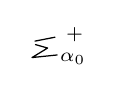
\begin{tikzpicture}[x=.055mm,y=-.055mm,baseline=(A021G10base),line cap=round,line join=round]
\path[use as bounding box] (620,1318) rectangle (758,1414);
\coordinate (A021G10base) at (620,1387);
\draw[line width=.45pt] (637,1349)--(683,1340);
\draw[line width=.45pt] (638,1357)--(666,1365)--(630,1387)--(688,1381);
\node[anchor=base west,inner sep=0pt,outer sep=0pt] at (695,1396) {$\scriptstyle\alpha_0$};
\node[anchor=base west,inner sep=0pt,outer sep=0pt] at (709,1346) {$\scriptstyle+$};
\end{tikzpicture}
% A021G10 END
% A021G11 BEGIN; source bbox=[777, 1327, 845, 1417]; source origin=(777,1327); baseline y=1378; owns: complete crossed inclusion, both strokes; neighbouring Sigmas outside
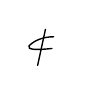
\begin{tikzpicture}[x=.055mm,y=-.055mm,baseline=(A021G11base),line cap=round,line join=round]
\path[use as bounding box] (777,1327) rectangle (845,1417);
\coordinate (A021G11base) at (777,1378);
% invisible complete reading/state annotation: \not\subset
\node[overlay,anchor=base west,inner sep=0pt,outer sep=0pt] at (777,1378) {\phantom{$\not\subset$}};
\draw[line width=.5pt] (837,1348)..controls(813,1348)and(793,1356)..(780,1369)..controls(775,1378)and(797,1379)..(833,1375);
\draw[line width=.5pt] (818,1331)--(800,1414);
\end{tikzpicture}
% A021G11 END
% A021G12 BEGIN; source bbox=[849, 1320, 953, 1401]; source origin=(849,1320); baseline y=1378; owns: complete Sigma, its separate head, index and any raised sign/hat; no adjoining relation or word
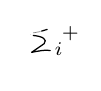
\begin{tikzpicture}[x=.055mm,y=-.055mm,baseline=(A021G12base),line cap=round,line join=round]
\path[use as bounding box] (849,1320) rectangle (953,1401);
\coordinate (A021G12base) at (849,1378);
\draw[line width=.45pt] (881,1328)--(894,1324);
\draw[line width=.45pt] (862,1338)..controls(884,1340)and(895,1347)..(887,1357)--(858,1377)..controls(873,1374)and(893,1370)..(901,1373);
\draw[gray,line width=.25pt] (862,1332)--(878,1329);
\fill[gray] (855,1336) circle[radius=.5];
\node[anchor=base west,inner sep=0pt,outer sep=0pt] at (911,1385) {$\scriptstyle i$};
\node[anchor=base west,inner sep=0pt,outer sep=0pt] at (928,1344) {$\scriptstyle+$};
\end{tikzpicture}
% A021G12 END
\]
ce qui $\unsure{% complete cancelled candidates impli / impl.; no expanded ending
% A021G21 BEGIN; source bbox=[588, 1428, 721, 1497]; source origin=(588,1428); baseline y=1471; owns: cancelled word only, including initial point, surviving loop and cancellation run; ce qui and live signifie outside
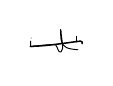
\begin{tikzpicture}[x=.055mm,y=-.055mm,baseline=(A021G21base),line cap=round,line join=round]
\path[use as bounding box] (588,1428) rectangle (721,1497);
\coordinate (A021G21base) at (588,1471);
% invisible complete reading/state annotation: \deleted{\text{impli}}\mid\deleted{\text{impl.}}
\node[overlay,anchor=base west,inner sep=0pt,outer sep=0pt] at (588,1471) {\phantom{$\deleted{\text{impli}}\mid\deleted{\text{impl.}}$}};
\draw[line width=.35pt] (595,1459)--(595,1472)..controls(615,1469)and(636,1467)..(652,1467)..controls(658,1473)and(658,1487)..(665,1484)..controls(673,1476)and(666,1458)..(665,1436)..controls(664,1428)and(663,1432)..(665,1454)..controls(667,1475)and(682,1477)..(704,1479);
\fill (596,1452) circle[radius=1];
\draw[line width=.35pt] (701,1448)--(701,1461);
\draw[line width=.55pt] (594,1471)..controls(631,1471)and(683,1462)..(710,1459)..controls(715,1458)and(714,1464)..(714,1465);
\end{tikzpicture}
% A021G21 END
}
$ signifie aussi que
$% A021G13 BEGIN; source bbox=[302, 1559, 415, 1639]; source origin=(302,1559); baseline y=1625; owns: complete Sigma, its separate head, index and any raised sign/hat; no adjoining relation or word
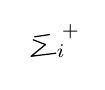
\begin{tikzpicture}[x=.055mm,y=-.055mm,baseline=(A021G13base),line cap=round,line join=round]
\path[use as bounding box] (302,1559) rectangle (415,1639);
\coordinate (A021G13base) at (302,1625);
\draw[line width=.45pt] (318,1580)--(352,1575);
\draw[line width=.45pt] (315,1587)--(343,1598)--(310,1625)--(367,1618);
\node[anchor=base west,inner sep=0pt,outer sep=0pt] at (369,1628) {$\scriptstyle i$};
\node[anchor=base west,inner sep=0pt,outer sep=0pt] at (381,1579) {$\scriptstyle+$};
\end{tikzpicture}
% A021G13 END
\cap% A021G14 BEGIN; source bbox=[452, 1564, 556, 1637]; source origin=(452,1564); baseline y=1612; owns: complete Sigma, its separate head, index and any raised sign/hat; no adjoining relation or word
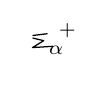
\begin{tikzpicture}[x=.055mm,y=-.055mm,baseline=(A021G14base),line cap=round,line join=round]
\path[use as bounding box] (452,1564) rectangle (556,1637);
\coordinate (A021G14base) at (452,1612);
\draw[line width=.45pt] (464,1582)--(497,1578);
\draw[line width=.45pt] (464,1588)--(489,1594)--(463,1610)--(510,1607);
\node[anchor=base west,inner sep=0pt,outer sep=0pt] at (501,1627) {$\scriptstyle\alpha$};
\node[anchor=base west,inner sep=0pt,outer sep=0pt] at (524,1582) {$\scriptstyle+$};
\end{tikzpicture}
% A021G14 END
=\varnothing$, cqfd.

\uline{Corollaire du lemme} Pour une classe
% The following left rule owns no text, and starts beneath the heading.
\noindent\begin{minipage}[t]{.04\linewidth}
$% A021G25 BEGIN; source bbox=[251, 1811, 277, 2343]; source origin=(251,1811); baseline y=2333; owns: corollary left vertical rule only; title and all words outside
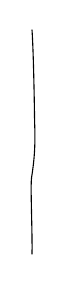
\begin{tikzpicture}[x=.055mm,y=-.055mm,baseline=(A021G25base),line cap=round,line join=round]
\path[use as bounding box] (251,1811) rectangle (277,2343);
\coordinate (A021G25base) at (251,2333);
\draw[line width=.4pt] (261,1816)..controls(264,1861)and(266,1954)..(267,2029)..controls(269,2078)and(267,2113)..(260,2157)..controls(257,2178)and(262,2277)..(261,2334);
\end{tikzpicture}
% A021G25 END
$
\end{minipage}\begin{minipage}[t]{.93\linewidth}
$overset{\unsure{% small pale point above V; role, hand and surface origin unresolved
% A021M03 BEGIN; source bbox=[321, 1836, 336, 1853]; source origin=(321,1836); baseline y=1848; owns: point only; V and de outside
\begin{tikzpicture}[x=.055mm,y=-.055mm,baseline=(A021M03base),line cap=round,line join=round]
\path[use as bounding box] (321,1836) rectangle (336,1853);
\coordinate (A021M03base) at (321,1848);
\fill[gray] (327,1843) ellipse[x radius=.5,y radius=1.2];
\end{tikzpicture}
% A021M03 END
}
}{V}$ de $% A021G22 BEGIN; source bbox=[490, 1863, 597, 1929]; source origin=(490,1863); baseline y=1907; owns: complete Pi, all separated/pale head pieces, lower I and ring; V de and comma outside
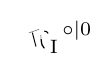
\begin{tikzpicture}[x=.055mm,y=-.055mm,baseline=(A021G22base),line cap=round,line join=round]
\path[use as bounding box] (490,1863) rectangle (597,1929);
\coordinate (A021G22base) at (490,1907);
% invisible complete reading/state annotation: \Pi_I^{\unsure{\circ|0}}
\node[overlay,anchor=base west,inner sep=0pt,outer sep=0pt] at (490,1907) {\phantom{$\Pi_I^{\unsure{\circ|0}}$}};
\draw[gray,line width=.25pt] (493,1875)--(516,1867);
\draw[line width=.35pt] (501,1875)--(509,1906);
\draw[gray,line width=.25pt] (520,1880)--(521,1888);
\draw[line width=.45pt] (521,1890)..controls(522,1901)and(524,1907)..(528,1910);
\draw[line width=.4pt] (529,1871)..controls(533,1871)and(536,1873)..(537,1876);
\node[anchor=base west,inner sep=0pt,outer sep=0pt] at (541,1923) {$\scriptstyle\mathrm I$};
\node[anchor=base west,inner sep=0pt,outer sep=0pt] at (570,1882) {$\scriptstyle\unsure{\circ|0}$};
\end{tikzpicture}
% A021G22 END
$, son expression
\[
V=X\setminus\bigcup_{\alpha\in K}
% A021G15 BEGIN; source bbox=[947, 1909, 1057, 1995]; source origin=(947,1909); baseline y=1978; owns: complete Sigma, its separate head, index and any raised sign/hat; no adjoining relation or word
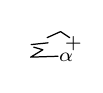
\begin{tikzpicture}[x=.055mm,y=-.055mm,baseline=(A021G15base),line cap=round,line join=round]
\path[use as bounding box] (947,1909) rectangle (1057,1995);
\coordinate (A021G15base) at (947,1978);
\draw[line width=.45pt] (955,1948)--(994,1944);
\draw[line width=.45pt] (961,1954)--(982,1960)--(954,1977)--(1017,1975);
\draw[line width=.45pt] (992,1932)--(1023,1918)--(1044,1932);
\node[anchor=base west,inner sep=0pt,outer sep=0pt] at (1019,1986) {$\scriptstyle\alpha$};
\node[anchor=base west,inner sep=0pt,outer sep=0pt] at (1033,1958) {$\scriptstyle+$};
\end{tikzpicture}
% A021G15 END
\]
du lemme pr\unsure{é|ê|e}c\unsure{é|e}dent est \uline{unique} -- on a
\[
% A021G24 BEGIN; source bbox=[463, 2225, 501, 2345]; source origin=(463,2225); baseline y=2298; owns: left brace only, through its surviving lower stem at the physical page edge; no unseen lower return
\begin{tikzpicture}[x=.055mm,y=-.055mm,baseline=(A021G24base),line cap=round,line join=round]
\path[use as bounding box] (463,2225) rectangle (501,2345);
\coordinate (A021G24base) at (463,2298);
\draw[line width=.4pt] (486,2230)..controls(486,2264)and(483,2287)..(477,2295)..controls(471,2298)and(463,2289)..(468,2289)..controls(483,2288)and(486,2302)..(489,2327)--(494,2344);
\end{tikzpicture}
% A021G24 END
\begin{aligned}K={}&\{\alpha\in I\mid\overline V\cap E_\alpha\ne\varnothing\quad\text{i.e.}\quad% A021G23 BEGIN; source bbox=[1422, 2182, 1504, 2263]; source origin=(1422,2182); baseline y=2247; owns: overwritten V and live E-alpha together; i.e., intersection and dotted V outside
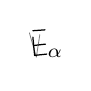
\begin{tikzpicture}[x=.055mm,y=-.055mm,baseline=(A021G23base),line cap=round,line join=round]
\path[use as bounding box] (1422,2182) rectangle (1504,2263);
\coordinate (A021G23base) at (1422,2247);
% invisible complete reading/state annotation: \deleted V E_\alpha
\node[overlay,anchor=base west,inner sep=0pt,outer sep=0pt] at (1422,2247) {\phantom{$\deleted V E_\alpha$}};
\draw[gray,line width=.3pt] (1426,2194)--(1442,2250)--(1450,2198);
\draw[line width=.45pt] (1434,2204)--(1438,2246)--(1466,2243);
\draw[line width=.45pt] (1434,2189)--(1462,2187);
\draw[line width=.45pt] (1437,2223)--(1463,2220);
\node[anchor=base west,inner sep=0pt,outer sep=0pt] at (1468,2250) {$\scriptstyle\alpha$};
\end{tikzpicture}
% A021G23 END
\cap\dot V\ne\varnothing\}\\% A021G16 BEGIN; source bbox=[525, 2297, 635, 2345]; source origin=(525,2297); baseline y=2341; owns: complete Sigma, its separate head, index and any raised sign/hat; no adjoining relation or word
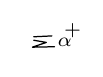
\begin{tikzpicture}[x=.055mm,y=-.055mm,baseline=(A021G16base),line cap=round,line join=round]
\path[use as bounding box] (525,2297) rectangle (635,2345);
\coordinate (A021G16base) at (525,2341);
\draw[line width=.45pt] (539,2318)--(581,2316);
\draw[line width=.45pt] (539,2326)--(568,2331)--(536,2342)--(587,2341);
\node[anchor=base west,inner sep=0pt,outer sep=0pt] at (594,2340) {$\scriptstyle\alpha$};
\node[anchor=base west,inner sep=0pt,outer sep=0pt] at (609,2315) {$\scriptstyle+$};
\end{tikzpicture}
% A021G16 END
&\ \text{est l'unique comp. de }X\setminus% A021G17 BEGIN; source bbox=[1156, 2290, 1216, 2340]; source origin=(1156,2290); baseline y=2326; owns: complete Sigma, its separate head, index and any raised sign/hat; no adjoining relation or word
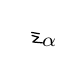
\begin{tikzpicture}[x=.055mm,y=-.055mm,baseline=(A021G17base),line cap=round,line join=round]
\path[use as bounding box] (1156,2290) rectangle (1216,2340);
\coordinate (A021G17base) at (1156,2326);
\draw[line width=.45pt] (1165,2301)--(1183,2304);
\draw[line width=.45pt] (1166,2308)--(1181,2312)--(1168,2323)--(1190,2325);
\node[anchor=base west,inner sep=0pt,outer sep=0pt] at (1189,2334) {$\scriptstyle\alpha$};
\end{tikzpicture}
% A021G17 END
\ \text{contenue dans }X\setminus V
\end{aligned}
\]
\end{minipage}
% archive sheet number: 20
